\documentclass[../final_report.tex]{subfiles}
\usepackage{subfiles}
\usepackage{diagbox}
\graphicspath{{../../Lab6/plots/}}
\begin{document}

Κέντρο της συγκεκριμένης άσκησης ήταν η επίλυση του προβλήματος της διάδοσης της θερμότητας
και συγκεκριμένα 3 από τις μεθόδους/αλγορίθμους που χρησιμοποιούνται για την επίλυση μερικών
διαφορικών εξισώσεων.

Η επίλυση της εξίσωσης διάδοσης της θερμότητας θα γίνει σε αρχιτεκτονικές κατανεμημένης μνήμης
με χρήση προγραμματιστικού μοντέλου MPI.

\subsection{Περιγραφή των μεθόδων}

Κάθε μέθοδος εκτελείται πάνω σε έναν 2D-πίνακα διαστάσεων MxN. Διατρέχουμε ολόκληρο τον πίνακα, στοιχείο-στοιχείο για να υπολογίσουμε την τρέχουσα
τιμή του πίνακα. 

\subsubsection{Μέθοδος Jacobi}
Η πιο απλή μέθοδος επίλυσης της διαφορικής εξίσωσης μετάδοσης θερμότητας. Για κάθε σημείο, παίρνουμε κατά μέσο όρο το άθροισμα των 4 γειτονικών σημείων. 
Αυτή η διαδικασία επαναλαμβάνεται "χρονικά" μέχρι να συγκλίνει η μέθοδος.

\begin{lstlisting}
void Jacobi(double ** u_previous, double ** u_current, int X_min, int X_max, int Y_min, int Y_max) {
	int i,j;
	for (i=X_min;i<X_max;i++)
		for (j=Y_min;j<Y_max;j++)
			u_current[i][j]=(u_previous[i-1][j]+u_previous[i+1][j]+u_previous[i][j-1]
            +u_previous[i][j+1])/4.0;
}
\end{lstlisting}

\subsubsection{Μέθοδος Gauss-Seidel με χρήση Successive Over-Relaxation}
Προχωράμε στην χρήση της μεθόδου successive over-relaxation, η οποία χρησιμοποιείται για να αυξήσουμε τον ρυθμό σύγκλισης σε iterative διεργασίες. 

Εκμεταλευόμαστε το γεγονός ότι σε κάθε σημείο, οι γείτονες σε θέση west,north έχουν ήδη υπολογίσει την τιμή τους για την παρούσα χρονική στιγμή. Άρα, αντί
να χρησιμοποιήσουμε και από τους 4 γείτονες τις τιμές της προηγούμενης χρονικής στιγμής, χρησιμοποιούμε την τιμή της παρούσας χρονικής στιγμής όπου είναι δυνατό.
Αυτό, μαζί με την χρήση του relaxation factor omega, προσφέρει πολύ καλύτερη επίδοση στο θέμα της σύγκλισης. 

\begin{lstlisting}
void GaussSeidel(double ** u_previous, double ** u_current, int X_min, int X_max, int Y_min, int Y_max, double omega) {
	int i,j;
	for (i=X_min;i<X_max;i++)
		for (j=Y_min;j<Y_max;j++)
			u_current[i][j]=u_previous[i][j]+(u_current[i-1][j]+u_previous[i+1][j]
            +u_current[i][j-1]+u_previous[i][j+1]-4*u_previous[i][j])*omega/4.0;
}
\end{lstlisting}

\subsubsection{Μέθοδος Red-Black oredring με χρήση Successive Over-Relaxation}

Η μέθοδος αυτή εκτελείται σε 2 φάσεις. Στην πρώτη φάση, υπολογίζουμε τις τιμές του πίνακα που βρίσκονται σε άρτια θέση (Update red phase) χρησιμοποιώντας
τις γειτονικές τιμές της προηγούμενης χρονικής στιγμής. 

Στην επόμενη φάση (Update black phase) υπολογίζουμε τις τιμές του πίνακα που βρίσκονται σε περιττή θέση χρησιμοποιώντας τις γειτονικές τιμές της παρούσας 
χρονικής στιγμής. Αυτό είναι εφικτό αφού όλοι οι γείτονες μιας περιττής θέσης (black) θα είναι τιμές που βρίσκονται σε άρτιες θέσεις (red).

Η μέθοδος αυτή προσφέρει καλύτερο ρυθμό σύγκλισης συγκριτικά με την Gauss-Seidel αλλά έχει 2 στάδια υπολογισμού αντί για 1.

\begin{lstlisting}
void RedSOR(double ** u_previous, double ** u_current, int X_min, int X_max, int Y_min, int Y_max, double omega) {
	int i,j;
	for (i=X_min;i<X_max;i++)
		for (j=Y_min;j<Y_max;j++)
			if ((i+j)%2==0) 
				u_current[i][j]=u_previous[i][j]+(omega/4.0)*(u_previous[i-1][j]
                +u_previous[i+1][j]+u_previous[i][j-1]+u_previous[i][j+1]-4*u_previous[i][j]);		         
}

void BlackSOR(double ** u_previous, double ** u_current, int X_min, int X_max, int Y_min, int Y_max, double omega) {
	int i,j;
	for (i=X_min;i<X_max;i++)
		for (j=Y_min;j<Y_max;j++)
			if ((i+j)%2==1) 
				u_current[i][j]=u_previous[i][j]+(omega/4.0)*(u_current[i-1][j]
                +u_current[i+1][j]+u_current[i][j-1]+u_current[i][j+1]-4*u_previous[i][j]); 
}
\end{lstlisting}

\subsection{Data Parallelism Pattern - Single Program Mulitple Data}

Για τις παράλληλες υλοποιήσεις που δημιουργήσαμε, ακολουθήσαμε την τεχνική της παραλληλοποίησης δεδομένων. Συγκεκριμένα, ακολουθήσαμε
την προσέγγιση Single Program Mulitple Data (SPMD). Στην προσέγγιση αυτή, όλες οι διεργασίες εκτελούν το ίδιο πρόγραμμα, αλλά υπάρχουν διαφορές
στην επικοινωνία και στα δεδομένα που επεξεργάζεται ο καθένας αναλόγως κάποιου χαρακτηριστικού ID που έχει κάθε διεργασία. Η τεχνική αυτή έχει προοπτικές
για πολύ καλή κλιμάκωση σε αρχιτεκτονικές κατανεμημένης μνήμης με χρήση προγραμματιστικού μοντέλου MPI. 

Η κύρια διεργασία, με PID=0 είναι αυτή η οποία κάνει τον διαμοιρασμό των δεδομένων στις υπόλοιπες διεργασίες και αργότερα λαμβάνει τα τελικά
αποτελέσματα από όλους.

Για να ξεκινήσουμε την διαδικασία του διαμοιρασμού, χωρίζουμε τον αρχικό πίνακα σε Grid, βάσει των διαθέσιμων διεργασιών που έχουμε σε κάθε εκτέλεση. Τις διαστάσεις
αυτού του grid τις ορίζουμε παραμετρικά από τις εισόδους Px,Py κατά την εκτέλεση του προγράμματος. Το γινόμενο Px*Py πρέπει πάντα να είναι
ίσο με των αριθμό MPI διεργασιών που έχουμε ορίσει.

Αν μπορούμε να διαιρέσουμε τέλεια την διάσταση globalX του πίνακα με τον αριθμό Px τότε η διάσταση localX του τοπικού block κάθε διεργασίας είναι ίσο με: $$  localX = \frac{globalX}{Px}$$ 
Αντίστοιχα βρίσκουμε την διάσταση localY του τοπικού block $$ localY = \frac{globalY}{Py} $$

Αν οι διαστάσεις globalX, globalY δεν διαιρούνται τέλεια τότε προσθέτουμε padding στον global πίνακα για ευκολία στον διαμοιρασμό. Θέλει ιδιαίτερη προσοχή αυτή η περίπτωση γιατί
κατά την διάρκεια του υπολογισμού, οι διεργασίες που κατέχουν εν τέλει dummy δεδομένα padding, ΔΕΝ πρέπει να τα λάβουν υπόψιν τους στους υπολογισμούς. 

Κάθε διεργασία λαμβάνει ένα υπό-block, διαστάσεων localX x localY. Ο διαμοιρασμός αυτός γίνεται από την διεργασία master, με την χρήση της εντολής \textbf{MPI\_Scatterv}
και φαίνεται καλύτερα στο παρακάτω σχήμα.

\begin{figure}[H]
    \centering
    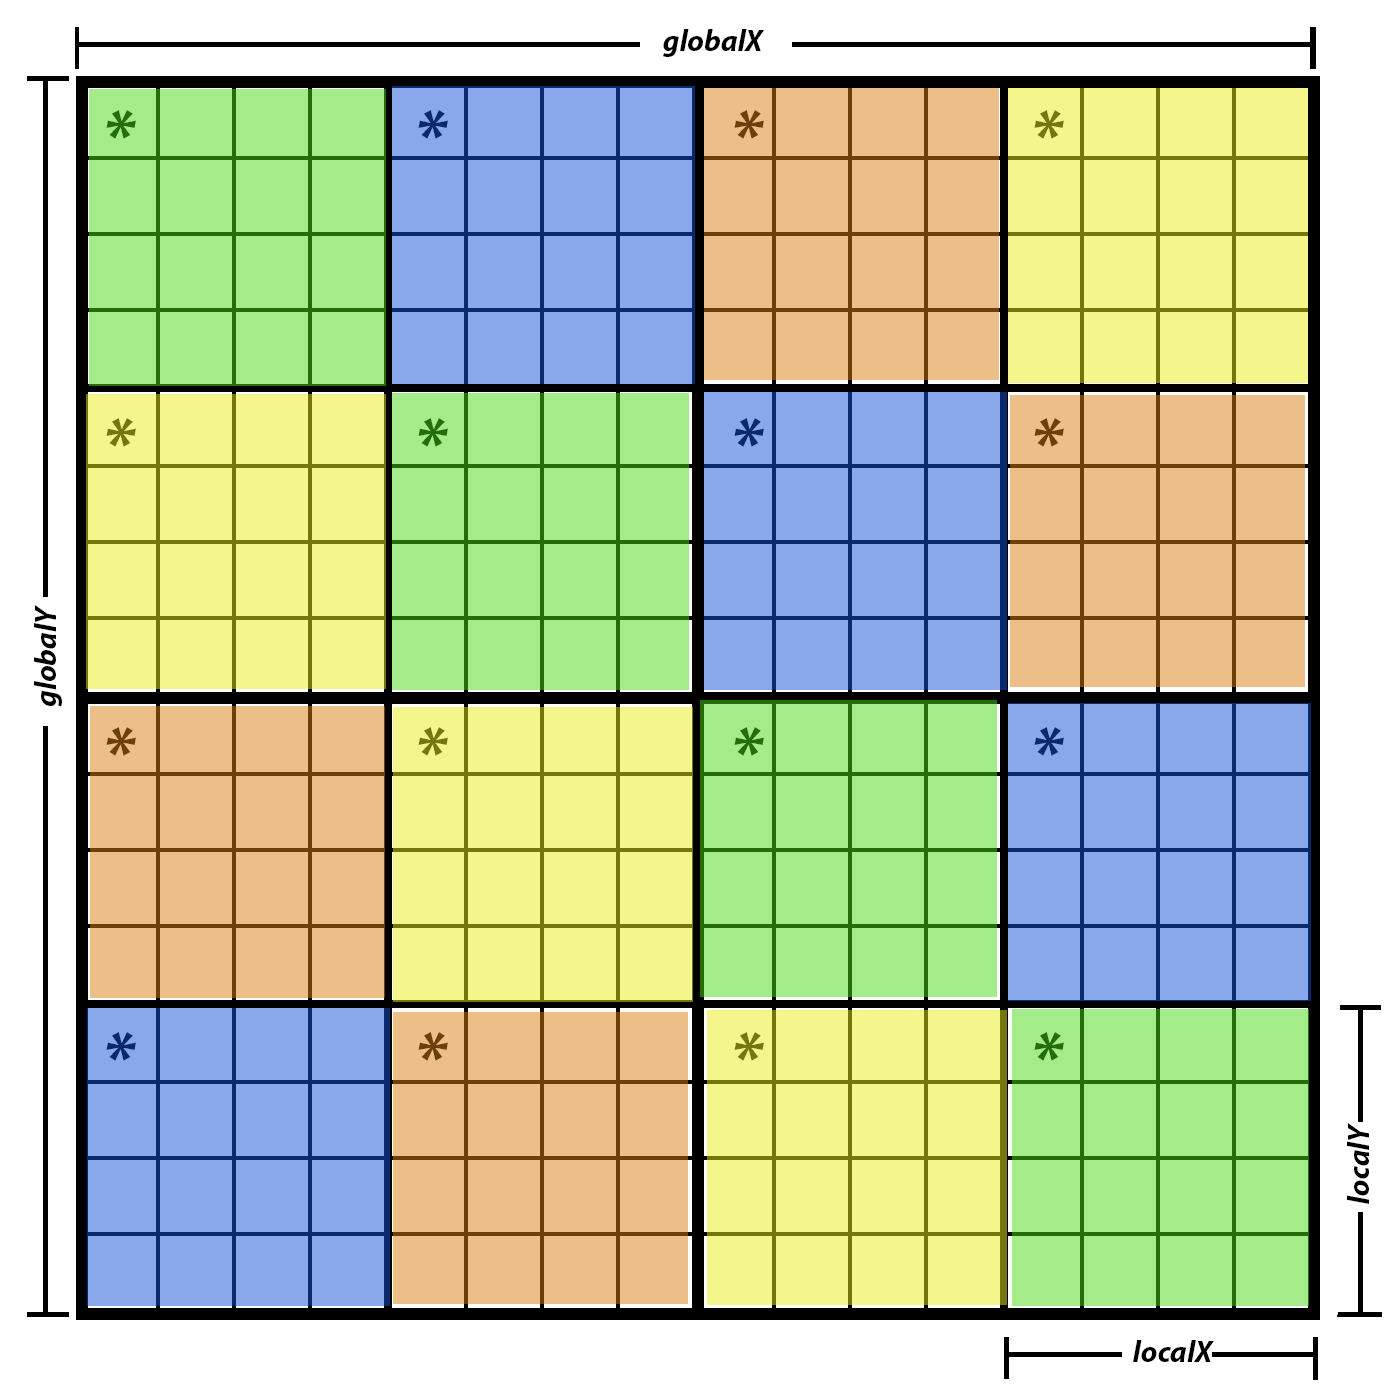
\includegraphics[scale=0.20]{global_block_scatter.png}
    \caption{Global and Local Blocks (16x16 Global - Px=4, Py=4)}
    \label{fig:Global and Local Blocks}
\end{figure}

Οι αστερίσκοι δείχνουν τα σημεία στα οποία ξεκινάει ο διαμοιρασμός δεδομένων (scatterpoints).

Η διαδικασία αυτή επαναλαμβάνεται ανάποδα, με χρήση της συνάρτησης \textbf{MPI\_Gatherv}, στο τέλος της εκτέλεσης του προγράμματος ώστε η master διεργασία
να λάβει τα αποτελέσματα πίσω στον global πίνακα.

\subsection{Ζητήματα επικοινωνίας μεταξύ διεργασιών}

Έχοντας πλέον χωρίσει τα δεδομένα σε ένα δισδιάστατο πλέγμα, προκύπτει το πρόβλημα επικοινωνίας μεταξύ διεργασιών καθώς οι συνοριακές τιμές των κελιών
χρειάζονται δεδομένα που ανήκουν σε άλλη διεργασία για να εκτελέσουν τους υπολογισμούς τους. Η επικοινωνία αυτή αλλάζει από μέθοδο σε μέθοδο.

Η κάθε διεργασία εκτελεί υπολογισμούς σε δικό της block, συγκεκριμένων διαστάσεων. 

\begin{figure}[H]
    \centering
    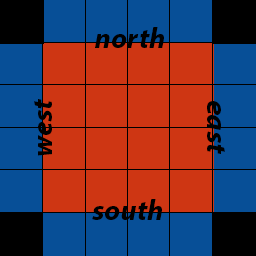
\includegraphics[scale=3]{local_block.png}
    \caption{Heat Transfer Methods - 4x4 Local Block}
    \label{fig:Heat Transfer Methods - Local Block}
\end{figure}

Κάθε block, έχει πραγματικές διαστάσεις NxN, αλλά έχουμε δεσμέυσει στην μνήμη διαστάσεις (N+2)x(N+2). Οι έξτρα θέσεις μνήμης αυτές είναι εκεί που θα 
στείλουν οι γειτονικές διεργασίες τα δεδομένα που χρειάζεται η κάθε διεργασία για τους υπολογισμούς του local block του.

Στο παραπάνω σχήμα, οι πραγματικές διαστάσεις του block παρουσιάζονται με κόκκινο χρώμα ενώ οι "βοηθητικές" θέσεις παρουσιάζονται με μπλε χρώμα. Τα 
μαύρα κουτάκια είναι δυναμικά δεσμευμένα, αλλά δεν χρησιμοποιούνται στο πρόβλημά μας.

Παρατηρούμε ότι επόμενη διαδικασία είναι η κάθε διεργασία να γνωρίζει ποιες διαδικασίες είναι οι γειτονικές του ώστε να γίνει σωστή ανταλλαγή δεδομένων.

Ο διαχωρισμός και η αποστολή δεδομένων στο OpenMPI μπορεί να γίνει με αρκετόυς τρόπους. Αξιοποιήσαμε την ύπαρξη των Cartesian Communicator. Η κάθε
διεργασία ανήκει σε συγκεκριμένη θέση στο δισδιάστατο πλέγμα, έχει ειδικό PID ίσο με το άθροισμα x+y όπου (x,y) οι διαστάσεις του στον Cartesian Communicator.

\begin{figure}[H]
    \centering
    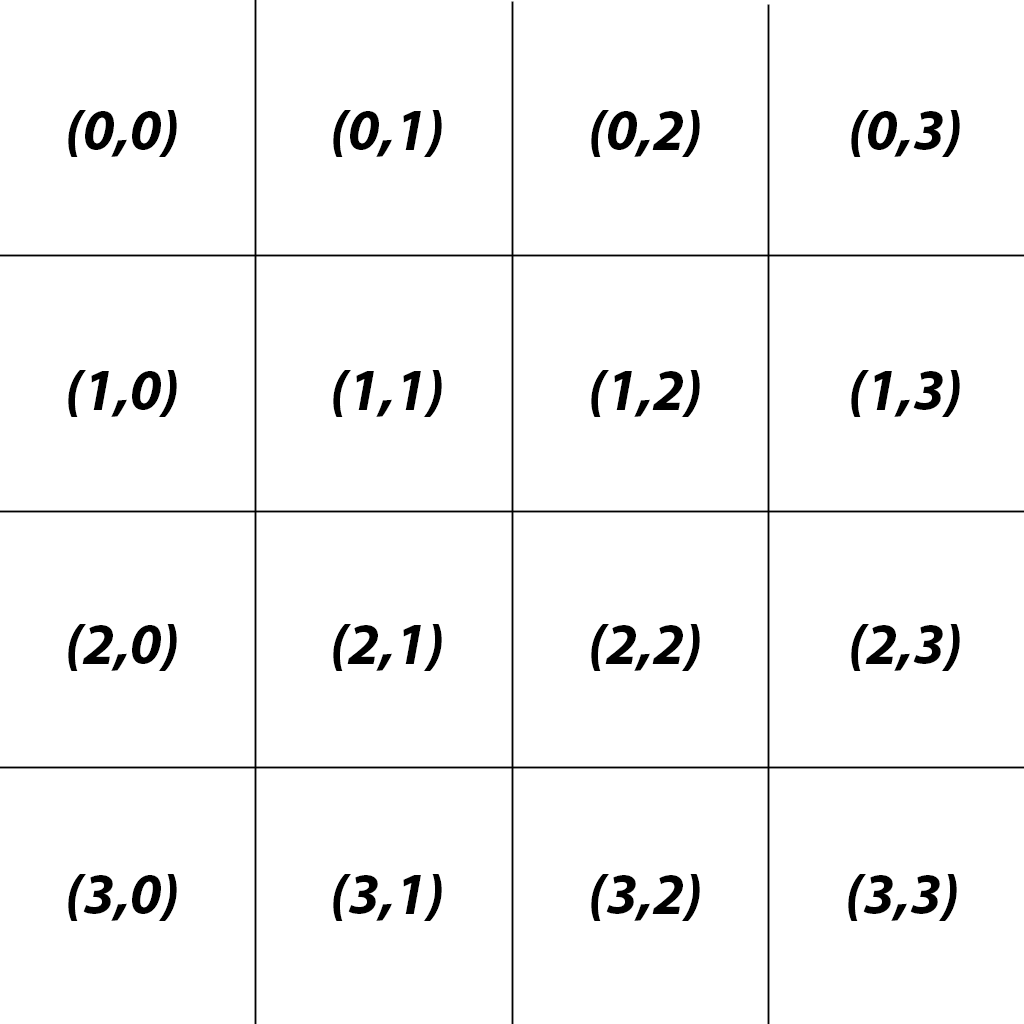
\includegraphics[scale=0.70]{cartesian_communicator.png}
    \caption{Heat Transfer Methods - Cartesian Communicator (Px=Py=4)}
    \label{fig:Heat Transfer Methods - Caertasian Communicator}
\end{figure}

Με χρήση της εντολής \textbf{MPI\_Cart\_shift}, η κάθε διεργασία μπορεί να βρεί τους west,east,north και south γείτονές της. Έτσι, η κάθε διεργασία γνωρίζει πλέον τους γείτονες τους
ή γνωρίζουν αν είναι συνοριακές διεργασίες, δηλαδή αν βρίσκονται στα άκρα του global πίνακα. 

\subsubsection*{Επικοινωνία στην μέθοδο Jacobi}
Για την μέθοδο Jacobi η επικοινωνία είναι αρκετά απλή. Κάθε διεργασία πρέπει να λάβει είτε μια στήλη πίνακα (από τους west, east γείτονες) ή μια γραμμή (από τους north, south γείτονες). 
Αντίστοιχα, η ίδια διεργασία πρέπει να στείλει τις γραμμές/στήλες που έχουν ανάγκη οι γειτονικές διεργασίες. 

Χρησιμοποιώντας το παραπάνω σχήμα που παρουσιάζουμε το local block, κάθε διεργασία πρέπει να αποστείλει στους αντίστοιχους γείτονές του τις κόκκινες στήλες/γραμμές και να λάβει από αυτούς
στις αντίστοιχες μπλε θέσεις τα δικά τους δεδομένα.

\begin{figure}[H]
    \centering
    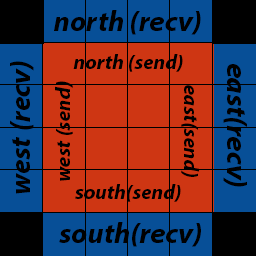
\includegraphics[scale=3]{jacobi-comm.png}
    \caption{Jacobi Communication - Each process sends to each neighbours the "send" row/column and receives the "recv" row/column}
    \label{fig:Jacobi Communication}
\end{figure}

Εφόσον υπάρχει αυτή η σχέση αποστολής/λήψης μηνύματος μεταξύ των γειτονικών διεργασιών, χρησιμοποιούμε την εντολή \textbf{MPI\_Sendrecv}. Οι οριακές
διεργασίες που δεν έχουν συγκεκριμένους γείτονες δεν παίρνουν μέρος στις επιμέρους επικοινωνίες. Η οποιαδήποτε διεργασία θα στείλει στην γειτονική της
και μετά θα μπλοκάρει μέχρι να λάβει από αυτή δεδομένα.

\subsubsection*{Επικοινωνία στην μέθοδο Gauss-Seidel}

Η επικοινωνία για την μέθοδο Gauss-Seidel είναι αρκετά διαφορετική καθώς πλέον γίνεται σε 2 φάσεις αντί για 1. Κάθε διεργασία, έχει ως dependency τιμές του 
πίνακα από τους αριστερούς και πάνω γείτονες (west,north).

\begin{figure}[H]
    \centering
    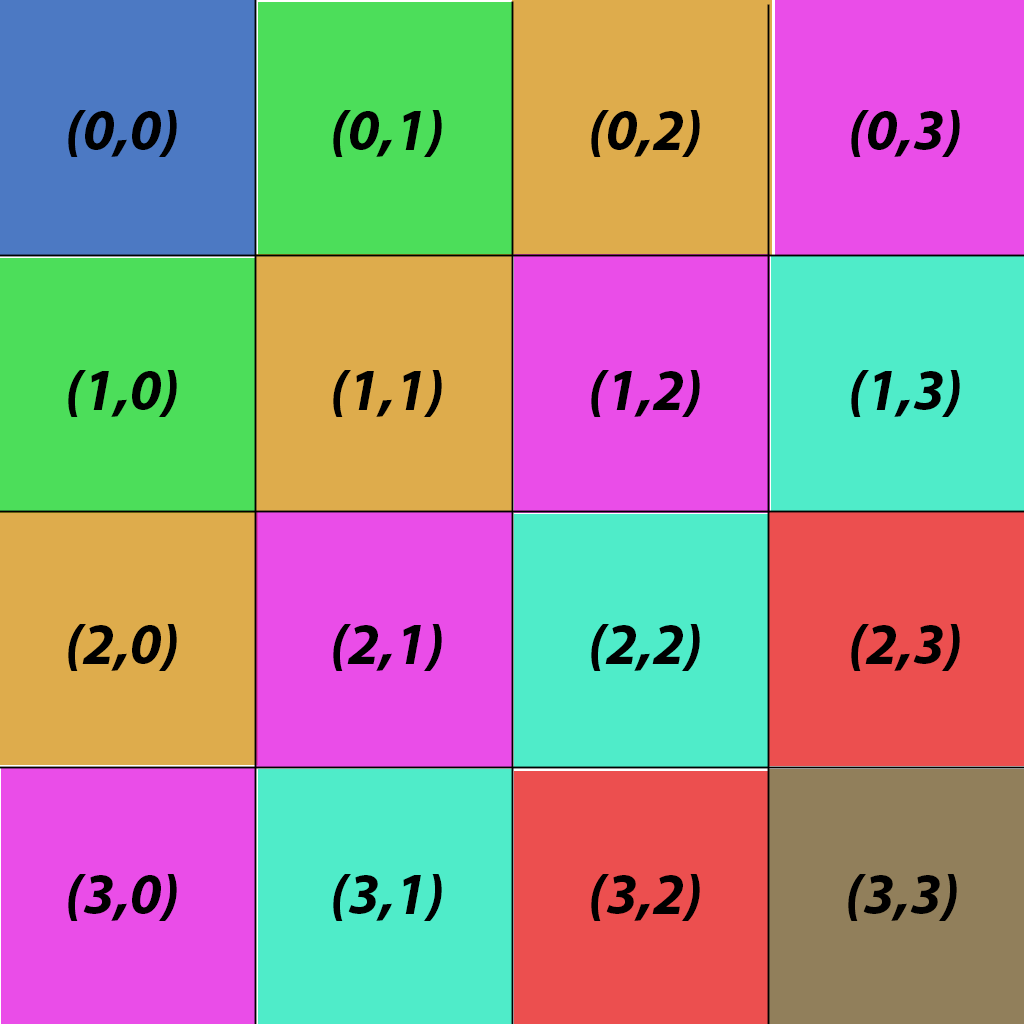
\includegraphics[scale=0.70]{gauss-seidel-comm.png}
    \caption{Heat Transfer Methods - Gauss-Seidel Communication (Px=Py=4)}
    \label{fig:Heat Transfer Methods - Gauss-Seidel Communication}
\end{figure}

Στο παραπάνω σχήμα φαίνεται με ποια σειρά μπορεί να γίνει η εκτέλεση της μεθόδου Gauss-Seidel. Οι διεργασίες με ίδιο χρώμα σημαίνει ότι μπορούν να τρέξουν ταυτόχρονα.
Η πρώτη διεργασία που μπορεί να ξεκινήσει τον υπολογισμό είναι (0,0) αφού δεν έχει κάποιο dependency από δεδομένα. Αφού υπολογιστεί όλο το block της (0,0) τότε μπορεί
να στείλει την οριακή east στήλη και south γραμμή ώστε να ξεκινήσουν τον υπολογισμό οι (1,0) και (0,1). Το μοτίβο αυτό επαναλαμβάνεται μέχρι να υπολογιστεί το τελευταίο 
block. 

Σε αντίθεση με την Jacobi, χρησιμοποιούμε τις non-blocking εκδοχές των send,recv. Στην εκτέλεση αυτών, επιστρέφεται ένα request στον χρήστη. Μαζέυοντας όλα τα request
για κάθε send/recv εντολή που χρησιμοποιεί η κάθε διεργασία για επικοινωνία με τους γείτονες, περιμένει στην ολοκλήρωση της επικοινωνίας στην εντολή \textbf{MPI\_Waitall}.

Άρα, οι διεργασίες που δεν έχουν κάποιο dependency, δηλαδή δεν περιμένουν στο request των receive, είναι ελεύθερα να εκτελέσουν τους υπολογισμούς τους.

Η διαδικασία επικοινωνίας του Gauss-Seidel είναι σίγουρα πιο περίπλοκη και χρονοβόρα από την Jacobi αλλά το αποτέλεσμα είναι ένας πολύ γρηγορότερος ρυθμός σύγκλισης.

\subsubsection*{Επικοινωνία στην μέθοδο Red-Black ordering}

Η επικοινωνία για την μέθοδο Red-Black είναι πολύ παρόμοια με αυτή του Jacobi. Η συγκεκριμένη, έχει 2 φάσεις υπολογισμού και 2 φάσεις επικοινωνίας.
Κάνουμε ανταλλαγή δεδομένων όπως κάναμε και στην Jacobi, αποστέλοντας τιμές του πίνακα της προηγούμενης χρονικής στιγμής και μετά εκτελούμε την φάση υπολογισμού
Update Red. Για την 2η φάση, κάνουμε την ίδια διαδκιασία επικοινωνίας, αυτή την φορά για τον πίνακα της παρούσας χρονικής στιγμής και μετά εκτελούμε την φάση υπολογισμού
Update Black. Είναι σαν να εκτελούμε 2 φορές την μέθοδο Jacobi.

Η μέθοδος Red-Black έχει το μεγαλύτερο overhead και από τους 3 αλγορίθμους, αλλά έχει και τον καλύτερο ρυθμό σύγκλισης.

\subsection{Μετρήσεις με έλεγχο σύγκλισης}

Κάποιες σύντομες σημειώσεις:
\begin{itemize}
    \item Ο χρόνος εκτέλεσης που υπολογίζουμε, είναι πάντα ο μέγιστος μεταξύ των διεργασιών
    \item Ο χρόνος επικοινωνίας είναι ο μέσος όρος μεταξύ της επικοινωνίας ΌΛΩΝ των διεργασιών
    \item Ο χρόνος σύγκλισης είναι επίσης ο μέγιστος μεταξύ όλων
\end{itemize}

Για κάθε αλγόριθμο που υλοποιήσαμε, κάναμε τις απαραίτητες μετρήσεις σε πίνακα μεγέθους 1024x1024, χρησιμοποιώντας 64 διεργασίες
MPI. Εξετάσαμε 3 διαφορετικούς συνδυασμούς για το grid size: 8x8, 16x4 και 4x16. Θα δούμε άμεσα ότι έχει πολύ μεγάλη σημασία
η επιλογή του σωστού block size.

\begin{figure}[H]
    \centering
    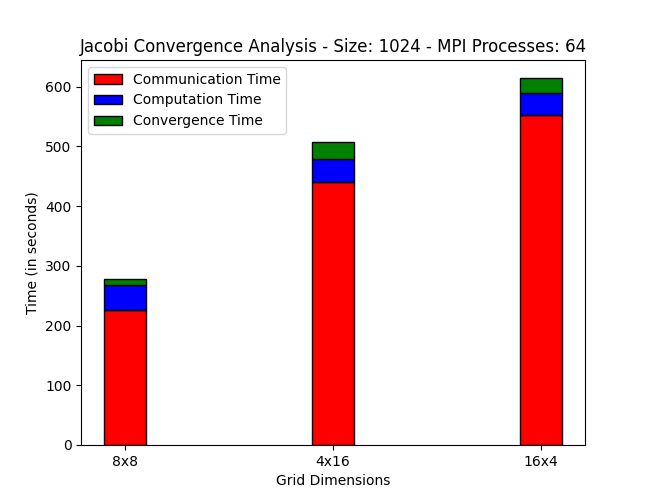
\includegraphics[scale=0.48]{/outFiles/plots/convergence/Jacobi_convergence_1024.png}
    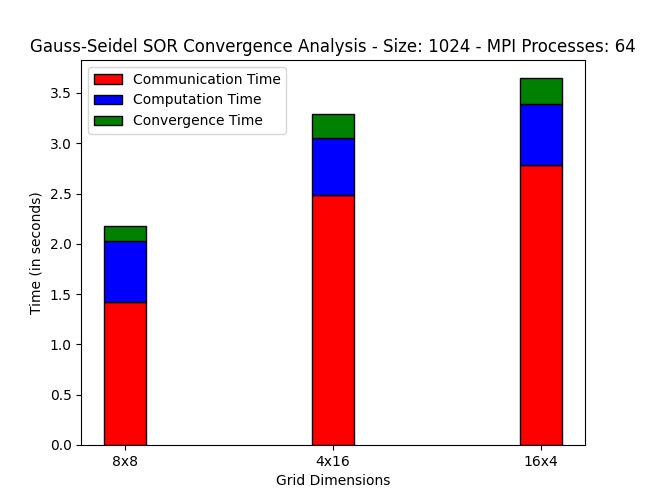
\includegraphics[scale=0.48]{/outFiles/plots/convergence/Gauss-Seidel SOR_convergence_1024.png}
    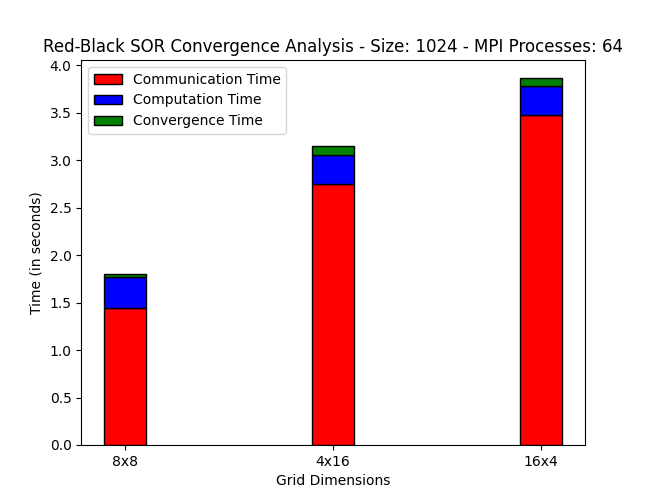
\includegraphics[scale=0.48]{/outFiles/plots/convergence/Red-Black SOR_convergence_1024.png}
    \caption{Heat Transfer Methods - Convergence Comparisson}
    \label{fig:Heat Transfer Methods - Convergence Comparisson}
\end{figure}

\noindent
\begin{tabular}{|l||*{6}{c|}}\hline
\backslashbox{Method}{Timers}
&\makebox[6.5em]{Communication}&\makebox[6.5em]{Computation}&\makebox[5em]{Convergence}&\makebox[5em]{Total}&\makebox[5em]{Iterations}
\\\hline\hline
Jacobi & 225.811780 & 40.527238 & 9.415624 & 270.395009 & 798200\\\hline
Gauss-Seidel SOR & 1.402382 & 0.604060 & 0.142405 & 2.109383 & 3200\\\hline
Red-Black SOR & 1.453022 & 0.327437 & 0.030029 & 1.829416 & 2500\\\hline
\end{tabular}
\hfill

\subsection*{Συμπεράσματα}

Η επιλογή του 8x8 grid size είναι ξεκάθαρη καθώς τα αποτελέσματα για 16x4 ή 4x16 είναι πολύ χειρότερα χωρίς να επηρεάζει κάπως αλλιώς
την ποιότητα του προγράμματος. Στα επόμενα πειράματα, χωρίς έλεγχο σύγκλισης, επιλέγουμε grid size 8x8 για τις εκτελέσεις με 64 διεργασίες.
 
\subsubsection*{Jacobi}
Ο Jacobi, καθώς είναι και η πιο naive λύση μαθηματικά αλλά και προγραμματιστικά, εχεί και την χειρότερη επίδοση. Το μεγαλύτερο μειονέκτημά του είναι
ο απίστευτα αργός ρυθμός σύγκλισης του. Χρειάζονται 250 φορές περισσότερα iterations συγκριτκά με τον Gauss Seidel και 320 φορές περισσότερα συγκριτκά με τον
Red-Black ordering.  

\subsubsection*{Gauss-Seidel SOR/Red-Black SOR}
Οι δύο αυτοί μέθοδοι ανήκουν στο ίδιο group καθώς οι επιδόσεις τους είναι πολύ παρόμοιες. Θεωρητικά, όπως θα δούμε και αργότερα, ο Gauss-Seidel έχει μικρότερο χρόνο
υπολογισμού καθώς γίνεται μόνο σε ένα μέρος του αλγορίθμου, σε αντίθεση με τον Red-Black που γίνεται σε 2 φάσεις. Όμως, ο Red-Black έχει το πλεονέκτημα ότι συγκλίνει
πιο γρήγορα. 

Τελικά, θα επιλέγαμε την μέθοδο Red-Black ordering για την επίλυση προβλημάτων που \textbf{ΑΠΑΙΤΟΥΝ} σύγκλιση.

\subsection{Μετρήσεις χωρίς έλεγχο σύγκλισης - Ποιοτικός έλεγχος scaling}
Για κάθε αλγόριθμο που υλοποιήσαμε, λαμβάνουμε μετρήσεις για μεγέθη πινάκων \{2048x2048, 4096x4096, 6144x6144\} και για \{1,2,4,8,16,32,64\}
διεργασίες MPI. Πλέον, δεν απαιτούμε σύγκλιση των μεθόδων, αλλά τρέχουμε και τους 3 αλγορίθμους για ακριβώς 256 iterations. Με αυτές τις μετρήσεις
θέλουμε να δούμε, ποιοτικά, πόσο καλά κλιμακώνουν οι μέθοδοι αυτοί.

\subsubsection{Speedup}

\begin{figure}[H]
    \centering
    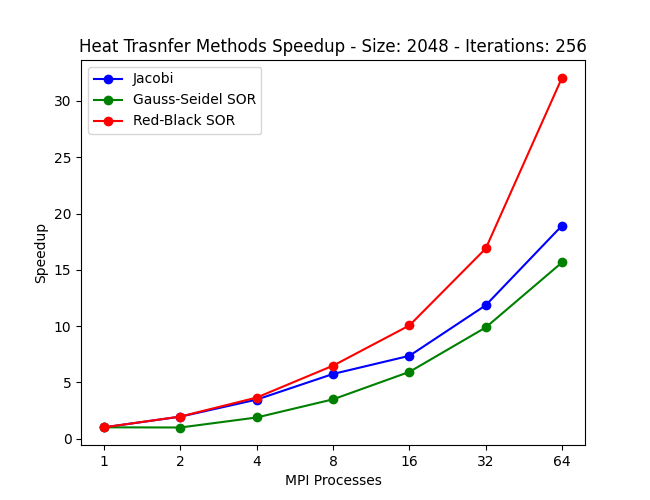
\includegraphics[scale=0.54]{/outFiles/plots/speedup/heat_transfer_2048_speedup.png}
    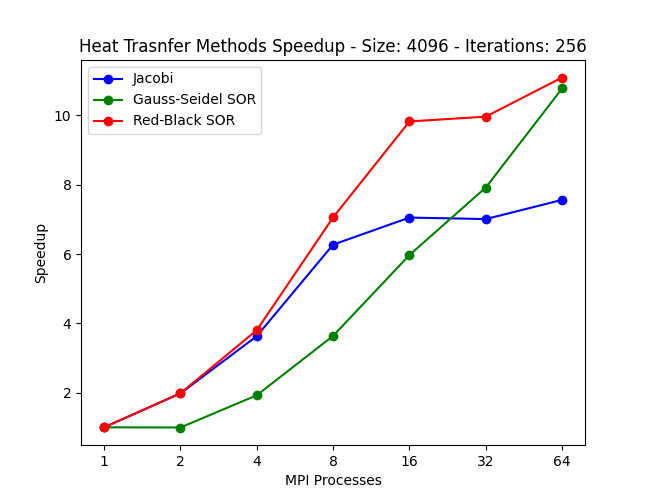
\includegraphics[scale=0.54]{/outFiles/plots/speedup/heat_transfer_4096_speedup.png}
    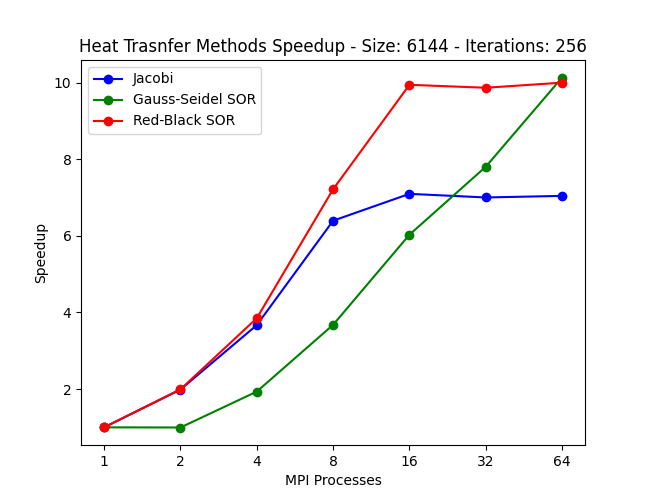
\includegraphics[scale=0.54]{/outFiles/plots/speedup/heat_transfer_6144_speedup.png}
    \caption{Heat Transfer Methods - Speedup}
    \label{fig:Heat Transfer MPI - Speedup}
\end{figure}

\subsubsection{Ανάλυση Χρόνου Εκτέλεσης}

\begin{figure}[H]
    \centering
    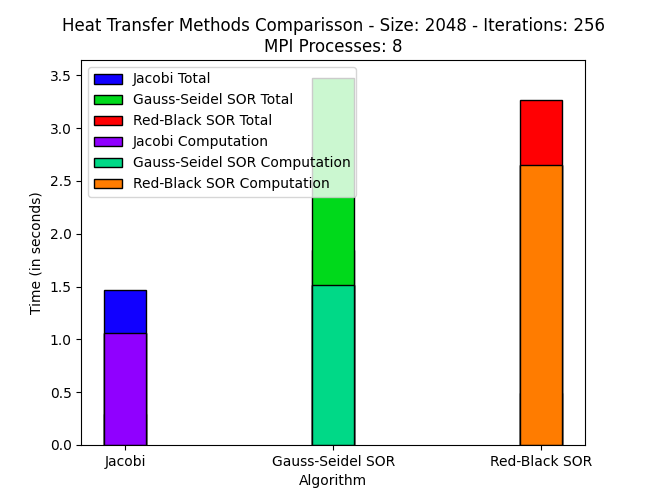
\includegraphics[scale=0.54]{/outFiles/plots/scaling/heat_transfer_comparisson_8_2048.png}
    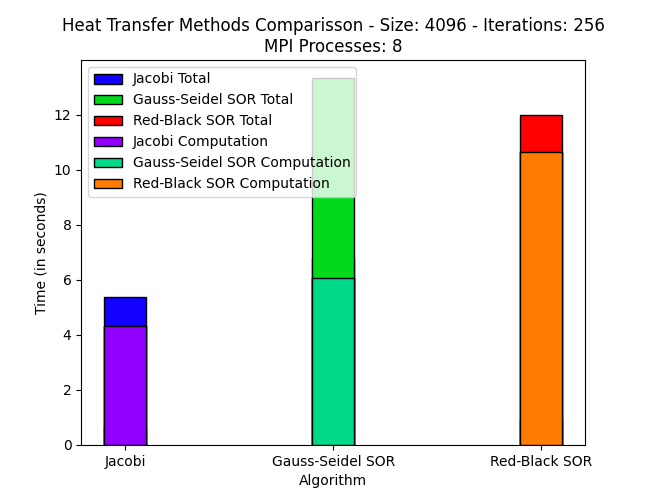
\includegraphics[scale=0.54]{/outFiles/plots/scaling/heat_transfer_comparisson_8_4096.png}
    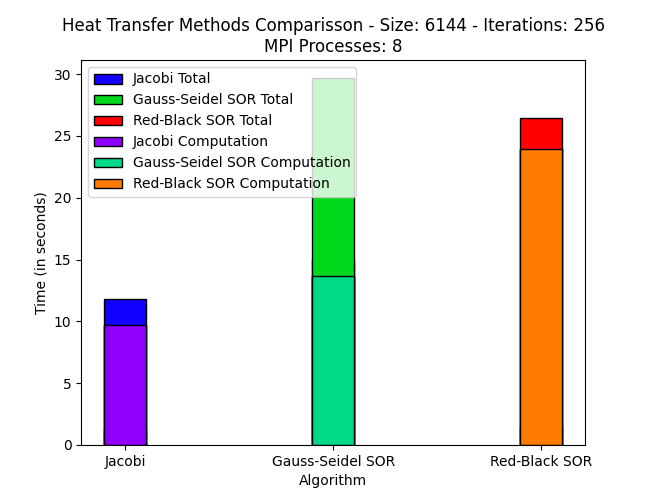
\includegraphics[scale=0.54]{/outFiles/plots/scaling/heat_transfer_comparisson_8_6144.png}
    \caption{Heat Transfer Methods - Time Comparisson - MPI Processes: 8}
    \label{fig:Heat Transfer Methods - Time Comparisson - MPI Processes: 8}
\end{figure}

\begin{figure}[H]
    \centering
    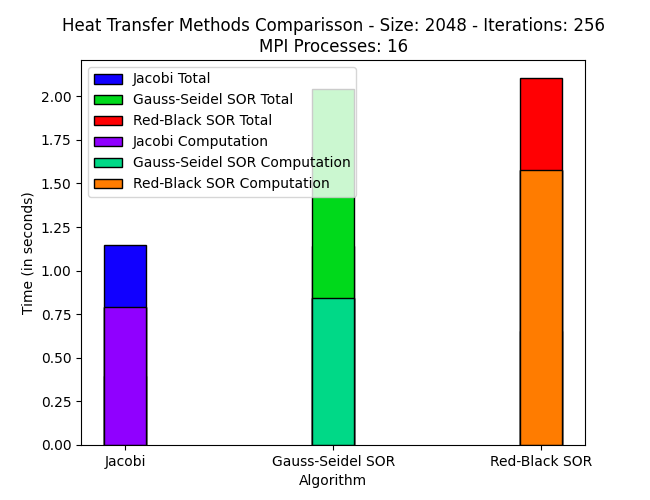
\includegraphics[scale=0.58]{/outFiles/plots/scaling/heat_transfer_comparisson_16_2048.png}
    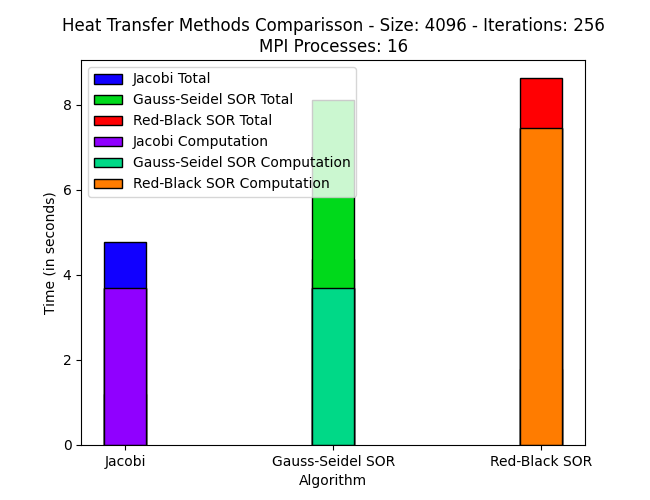
\includegraphics[scale=0.58]{/outFiles/plots/scaling/heat_transfer_comparisson_16_4096.png}
    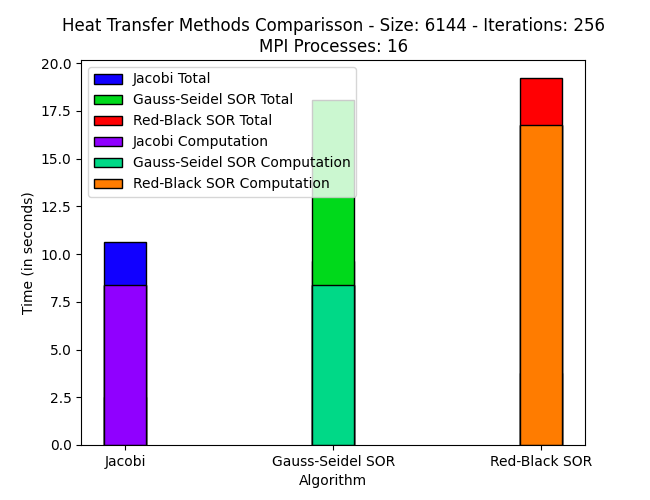
\includegraphics[scale=0.58]{/outFiles/plots/scaling/heat_transfer_comparisson_16_6144.png}
    \caption{Heat Transfer Methods - Time Comparisson - MPI Processes: 16}
    \label{fig:Heat Transfer Methods - Time Comparisson - MPI Processes: 16}
\end{figure}

\begin{figure}[H]
    \centering
    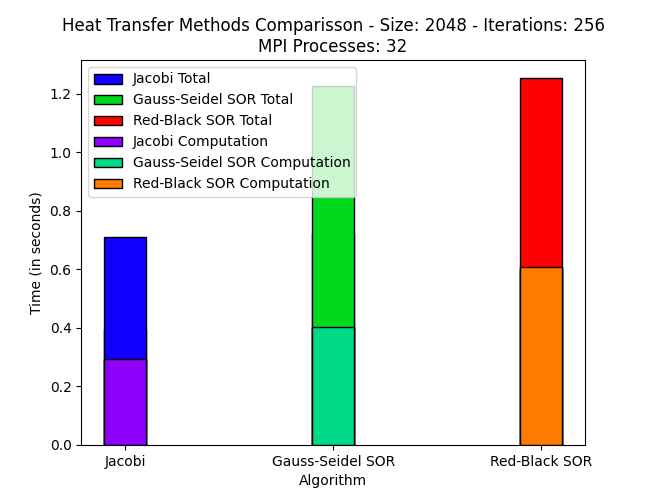
\includegraphics[scale=0.58]{/outFiles/plots/scaling/heat_transfer_comparisson_32_2048.png}
    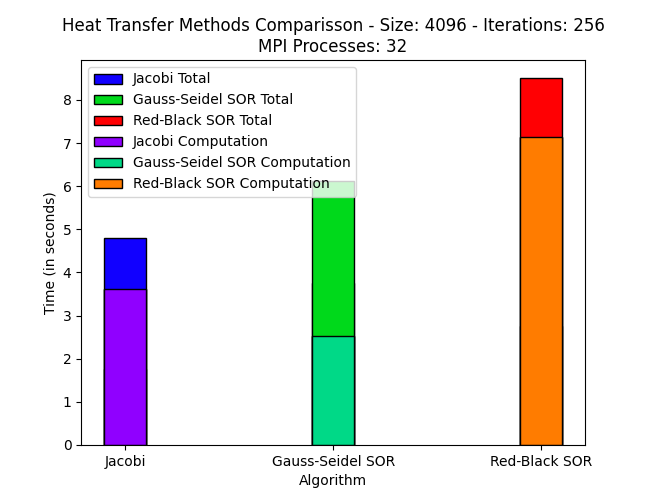
\includegraphics[scale=0.58]{/outFiles/plots/scaling/heat_transfer_comparisson_32_4096.png}
    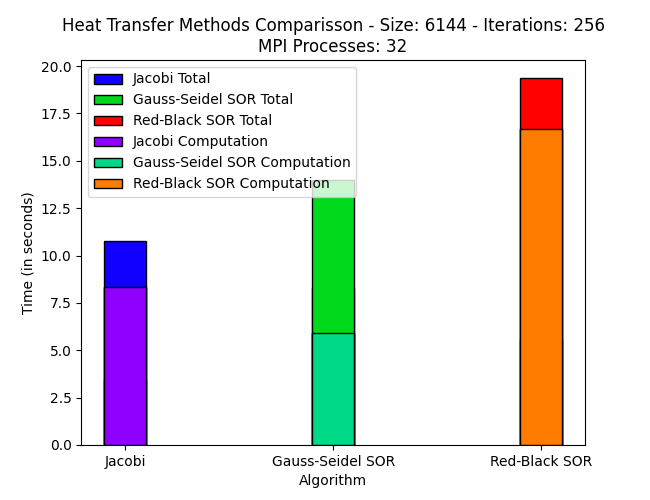
\includegraphics[scale=0.58]{/outFiles/plots/scaling/heat_transfer_comparisson_32_6144.png}
    \caption{Heat Transfer Methods - Time Comparisson - MPI Processes: 32}
    \label{fig:Heat Transfer Methods - Time Comparisson - MPI Processes: 32}
\end{figure}

\begin{figure}[H]
    \centering
    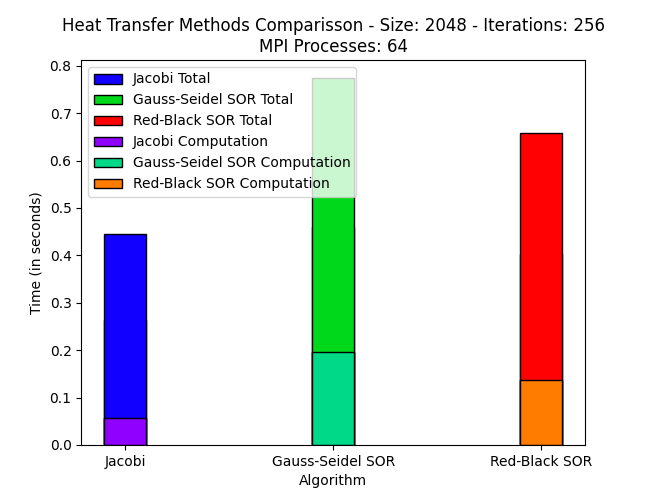
\includegraphics[scale=0.58]{/outFiles/plots/scaling/heat_transfer_comparisson_64_2048.png}
    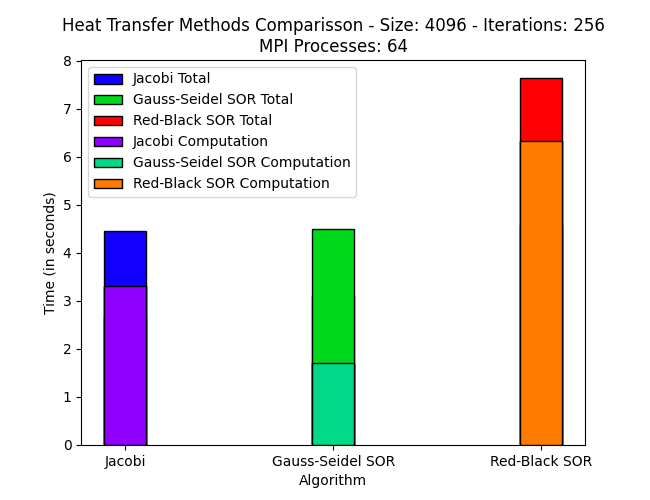
\includegraphics[scale=0.58]{/outFiles/plots/scaling/heat_transfer_comparisson_64_4096.png}
    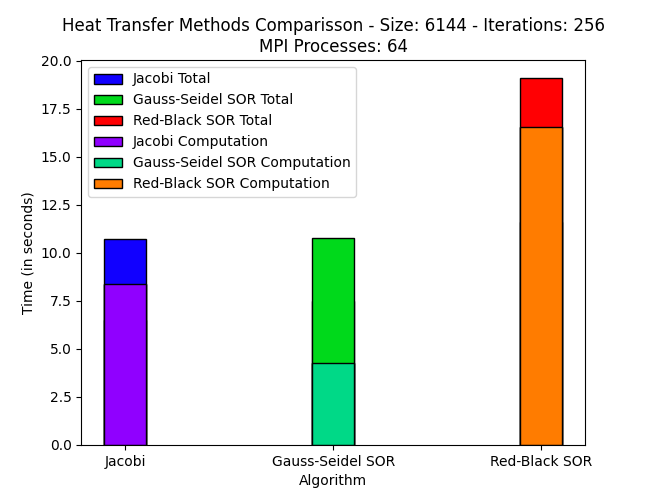
\includegraphics[scale=0.58]{/outFiles/plots/scaling/heat_transfer_comparisson_64_6144.png}
    \caption{Heat Transfer Methods - Time Comparisson - MPI Processes: 64}
    \label{fig:Heat Transfer Methods - Time Comparisson - MPI Processes: 64}
\end{figure}

\begin{figure}[H]
    \centering
    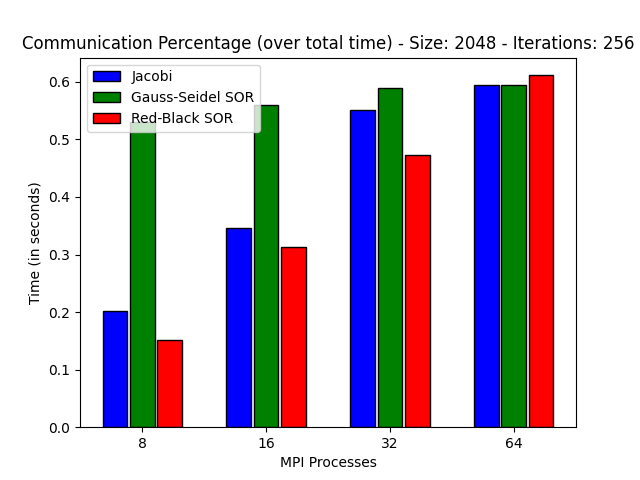
\includegraphics[scale=0.58]{/outFiles/plots/extras/heat_transfer_communication_analysis_2048.png}
    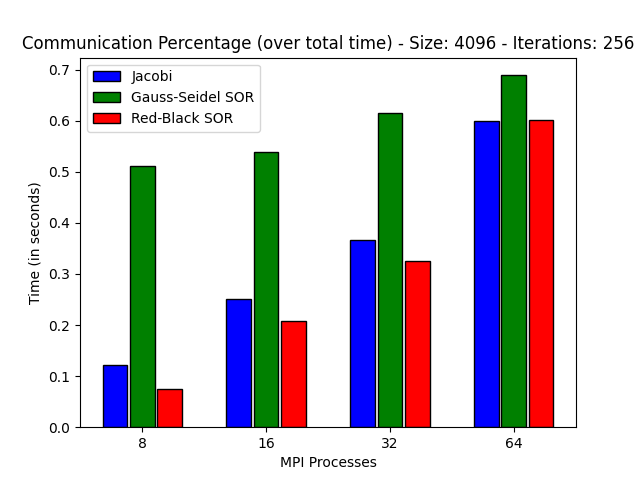
\includegraphics[scale=0.58]{/outFiles/plots/extras/heat_transfer_communication_analysis_4096.png}
    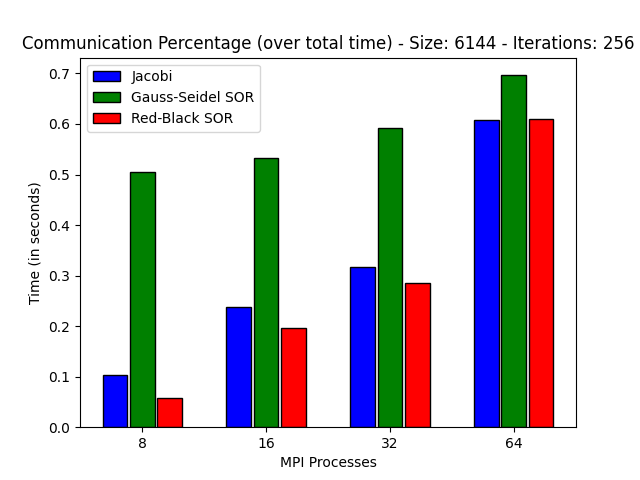
\includegraphics[scale=0.58]{/outFiles/plots/extras/heat_transfer_communication_analysis_6144.png}
    \caption{Heat Transfer Methods - Communication Analysis}
    \label{fig:Heat Transfer Methods - Communication Analysis}
\end{figure}

\begin{figure}[H]
    \centering
    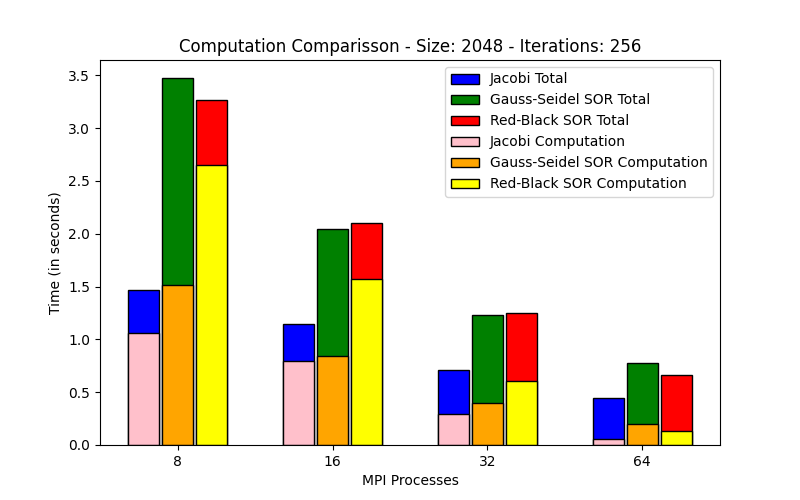
\includegraphics[scale=0.48]{/outFiles/plots/extras/heat_transfer_computation_analysis_2048.png}
    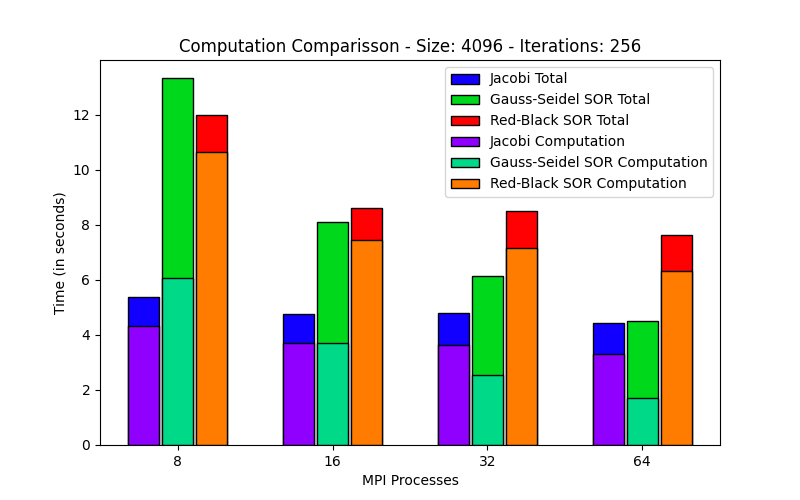
\includegraphics[scale=0.48]{/outFiles/plots/extras/heat_transfer_computation_analysis_4096.png}
    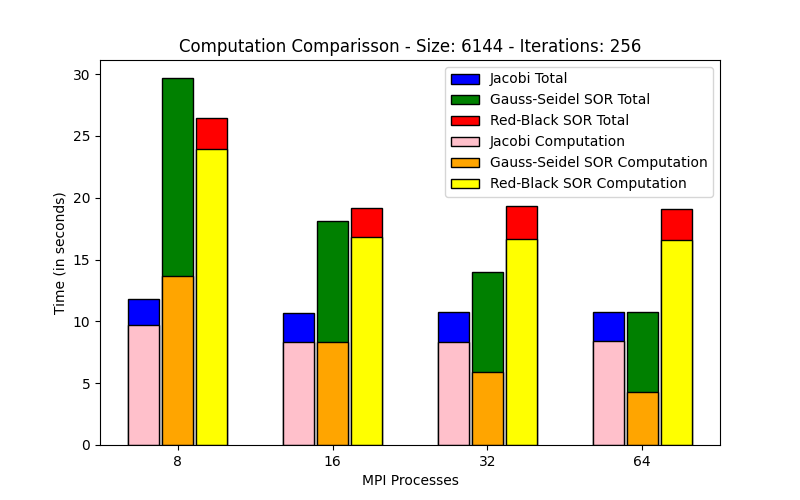
\includegraphics[scale=0.48]{/outFiles/plots/extras/heat_transfer_computation_analysis_6144.png}
    \caption{Heat Transfer Methods - Computation Analysis}
    \label{fig:Heat Transfer Methods - Computation Analysis}
\end{figure}

\subsection*{Συμπεράσματα}


Για πίνακα μεγέθους 2048x2048, και οι 3 μέθοδοι κλιμακώνουν με καλό ρυθμό.

Για πίνακες μεγέθους 4096x4096 και 6144x6144 παρατηρούμε λίγο διαφορετικά αποτελέσματα. Η μέθοδος Gauss-Seidel βελτιώνεται στις επιδόσεις της
με παρόμοιο ρυθμό στους διπλασιασμούς των διεργασιών και δεν φαίνεται να "σπαει". Αντιθέτως, οι Jacobi και Red-Black "σπάνε", η πρώτη μετά από τις 8 διεργασίες
και η δεύτερη από τις 16 και πάνω.

\end{document}